\documentclass{article}
\usepackage{../verslagstyle}


\begin{document}
	\title{Labo 1}
	\author{Bert De Saffel}
	\date{11 februari 2019}
	\maketitle
	
	\section{Oplosmethode}
	De opgave is opgelost met behulp van Python. Als eerste deel is er een minimale vorm van argument checking, om na te gaan of het opgegeven argument wel degelijk een bestand is. De controle dat het een effectieve image is wordt overgelaten aan OpenCV zelf. Het opgegeven argument wordt gesplitst zodat de extensie en het pad apart beschikbaar zijn. Het pad wordt gebruikt om een venster aan te maken met behulp van namedWindow, en de bestandsextensie wordt later gebruikt om de image terug weg te schrijven. 
	
	De rest van de code is het stapsgewijs uitvoeren van de labo-opdracht, met behulp van de functies in volgend onderdeel.
	\section{Gebruikte functies}
	\begin{itemize}
		\item \textbf{namedWindow(winname[, flags]) $\rightarrow$ None} 
		
		Maakt een venster aan met als naam de \textit{winname} parameter. De optionele \textit{flags} parameter geeft extra eigenschappen aan het venster. Deze functie heeft geen returntype, maar het aangemaakte venster kan wel aangesproken via de opgegeven \textit{winname} bij andere functies. Een eenvoudige keuze van \textit{winname} is de naam van het opgegeven bestand zelf.
		
		\item \textbf{imread(filename[, flags]) $\rightarrow$ retval}
		
		Probeert een foto te laden met het opgegeven \textit{filename}. Indien de \textit{filename} op het bestandssysteem staat wordt een referentie teruggeven naar een \textit{numpy.ndarray} object, een multidimensionale array die de eigenlijke image voorstelt. De optionele \textit{flags} parameter laat voornamelijk toe om kleurenconversies uit te voeren op de image. De default waarde is \texttt{IMREAD\_UNCHANGED}, die aangeeft dat de image onveranderd blijft.
		
		\item \textbf{imshow(winname, mat) $\rightarrow$ None}
		
		Zal een image, meegegeven met de \textit{mat} parameter, tonen in het venster met als naam \textit{winname}.
		
		
		\item \textbf{imwrite(filename, img[, params]) $\rightarrow$ retval}
		
		Zal een image, meegegeven met de \textit{img} parameter, opslaan naar een specifiek bestand, meegegeven met de \textit{filename} parameter. De optionele \textit{params} parameter bevat opties in de vorm van paren (paramId1, paramValue1, paramId2, paramValue2, ...). Deze opties hebben betrekking tot onder andere compressie en kwaliteit van de image.
		
		\item \textbf{cvtColor(src, code[, dst[, dstCn]]) $\rightarrow$ dst}
		
		Converteert een image van een kleurenruimte naar een andere. De \textit{src} parameter bevat de input image. De \textit{code} parameter bevat de conversieregel die gebruikt moet worden. In dit labo wordt de code \texttt{COLOR\_BGR2GRAY} gebruikt, om een kleurenbeeld in grijsschaal om te zetten. De conversie van een kleurenpixel naar een grijspixel kan door de de som te nemen van de individuele kleurencomponenten, elk vermenigvuldigt met een constante:
		$$Y \leftarrow 0.299 \cdot R + 0.587 \cdot G + 0.114 \cdot B$$
		waarbij Y de intensiteit van een willekeurige pixel voorstelt voor de grijsschaal image, en R, G en B de kleurencomponenten die horen tot die pixel van de originele image.
		
		Deze functie kan op twee manieren de grijsschaal image teruggeven: enerzijds via de returnwaarde \textit{dst} en anderzijds door de referentieparameter \textit{dst}. De eerste methode is handig voor als er nog geen image object beschikbaar is, of als er niet gewenst is om een bestaande image te overschrijven.
		
		\item \textbf{threshold(src, thresh, maxval, type[, dst]) $\rightarrow$ retval, dst}
		
		Past een threshold toe op de \textit{src} image. In dit labo wordt het \textit{type} ingesteld op \texttt{THRESH\_BINARY}. Dit komt neer op de stuksgewijze functie:
		\begin{equation*}
			dst(x, y) = \begin{cases}
			maxval &, src(x, y) > thresh\\
			0 &, src(x, y) \leq thresh
			\end{cases}
		\end{equation*}

		Om een zwart-wit image te genereren vanuit een grijsschaal image wordt \textit{maxval = 255} en \textit{thresh = 127} genomen. Voor een pixelintensiteit groter dan 127 wordt de intensiteit 255, wat overeenkomt met een witte pixel. Anderzijds voor een pixelintensiteit kleiner of gelijk dan 127 wordt de intensiteit 0, wat overeenkomt met een zwarte pixel. 
		
		Net zoals de functie \textit{cvtColor} heeft de \textit{threshold} functie dezelfde twee manieren om de uitvoer op te vangen. De \textit{retval} returnwaarde is enkel van belang indien \texttt{THRESH\_OTSU} of \texttt{THRESH\_TRIANGLE} gekozen wordt als waarde voor de parameter \textit{type}.
		
		\item \textbf{waitKey([, delay]) $\rightarrow$ retval}
		
		Deze functie wacht tot dat de gebruiker een knop heeft ingedrukt op zijn toetsenbord. Vaak wordt deze functie gebruikt in combinatie met de \textit{imshow} functie, aangezien anders de getoonde foto niet tevoorschijn komt. Het is ook mogelijk om een \textit{delay} op te geven, in milliseconden, die aangeeft hoe lang de functie zal wachten op antwoord van de gebruiker. Een delay $\leq 0$ zal oneindig lang wachten. De returnwaarde van deze functie is de code die overeenkomt met de ingedrukte toets.
		
		
	\end{itemize}

	\section{Invoer en uitvoer}
	Als testimage wordt de foto \textit{clouds.png} gebruikt. Figuur \ref{Fig:Data1}, \ref{Fig:Data2} en \ref{Fig:Data3} tonen respectievelijk de originele image, de grijsschaalimage en de binaire image.
	\begin{figure}[!htb]
		\begin{minipage}{0.3\textwidth}
			\centering
			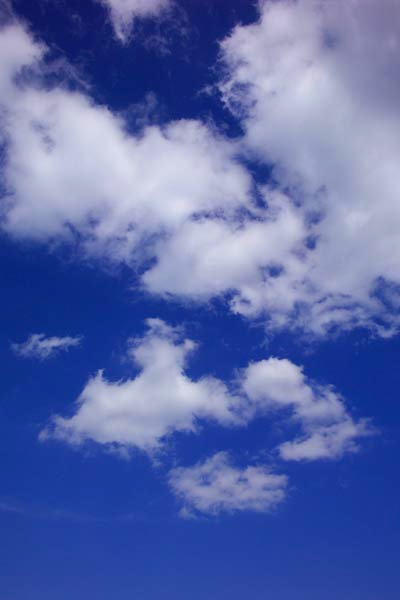
\includegraphics[width=0.9\linewidth]{clouds}
			\caption{De originele, onaangepaste image.}\label{Fig:Data1}
		\end{minipage}\hfill
		\begin{minipage}{0.3\textwidth}
			\centering
			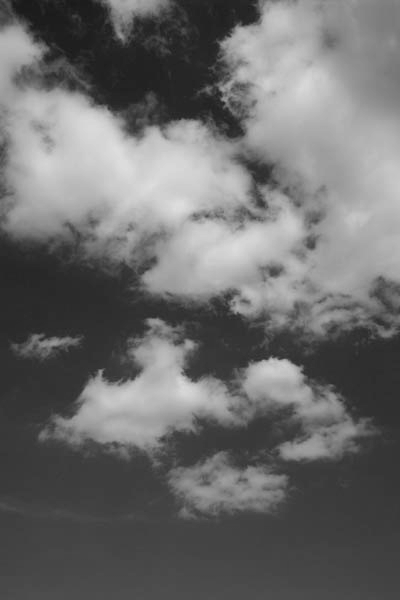
\includegraphics[width=0.9\linewidth]{cloudsGRAYSCALE}
			\caption{Figuur \ref{Fig:Data1} geconverteerd naar grijsschaal.}\label{Fig:Data2}
		\end{minipage}\hfill
		\begin{minipage}{0.3\textwidth}
			\centering
			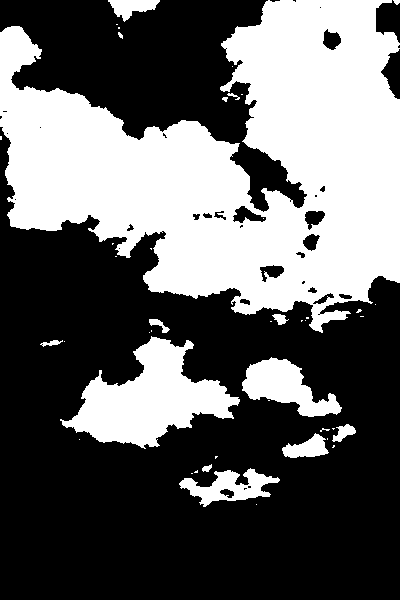
\includegraphics[width=0.9\linewidth]{cloudsTHRESHOLD}
			\caption{Binaire thresholding uitgevoerd op figuur \ref{Fig:Data2}.}\label{Fig:Data3}
		\end{minipage}
	\end{figure}

\end{document}